\section{Running example: a simple train controller system\label{section:background-running-example}}

We use a simple train system fragment as running example for illustrating concepts and techniques throughout this thesis. The system is composed of an automated train controller, actuators for doors and the engine as well as the latter themselves, sensors, and a passenger. Via the actuators, the controller typically controls operations like starting or stopping the train, opening or closing the doors, and so on. A safety goal requires train doors to remain closed while the train is moving. If the train is not moving and the passenger presses the alarm button, the controller must open the doors immediately. If the train is moving and the passenger presses the alarm button, then the controller must stop the train first and then open the doors. Typical agent interactions for the latter case are depicted in Fig.~\ref{image:train-scenario-all-agents}. The precise semantics of such a scenario is made clear in the following sections.

\begin{figure}\centering
\scalebox{0.75}{
  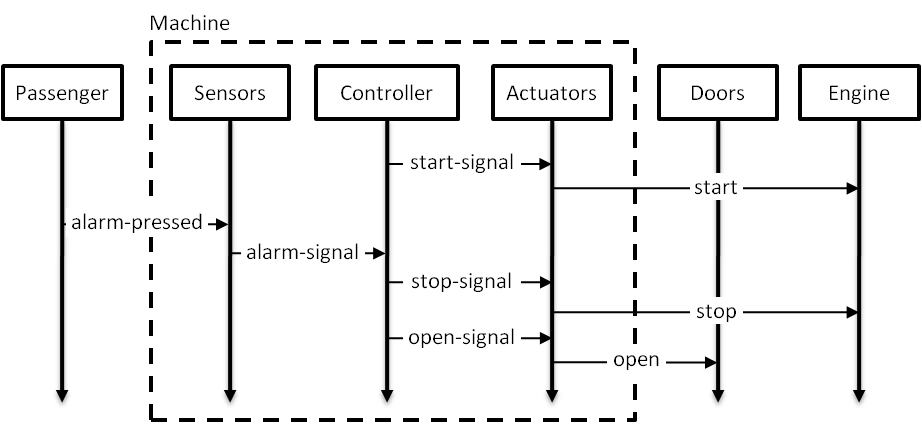
\includegraphics[trim=2mm 2mm 2mm 2mm, clip]{src/2-framework/images/train-scenario-all-agents}
}
\caption{A scenario illustrating a train system stopping in emergency when an alarm is pressed.\label{image:train-scenario-all-agents}}
\end{figure}

